\begin{figure}[!t]
    \centering
    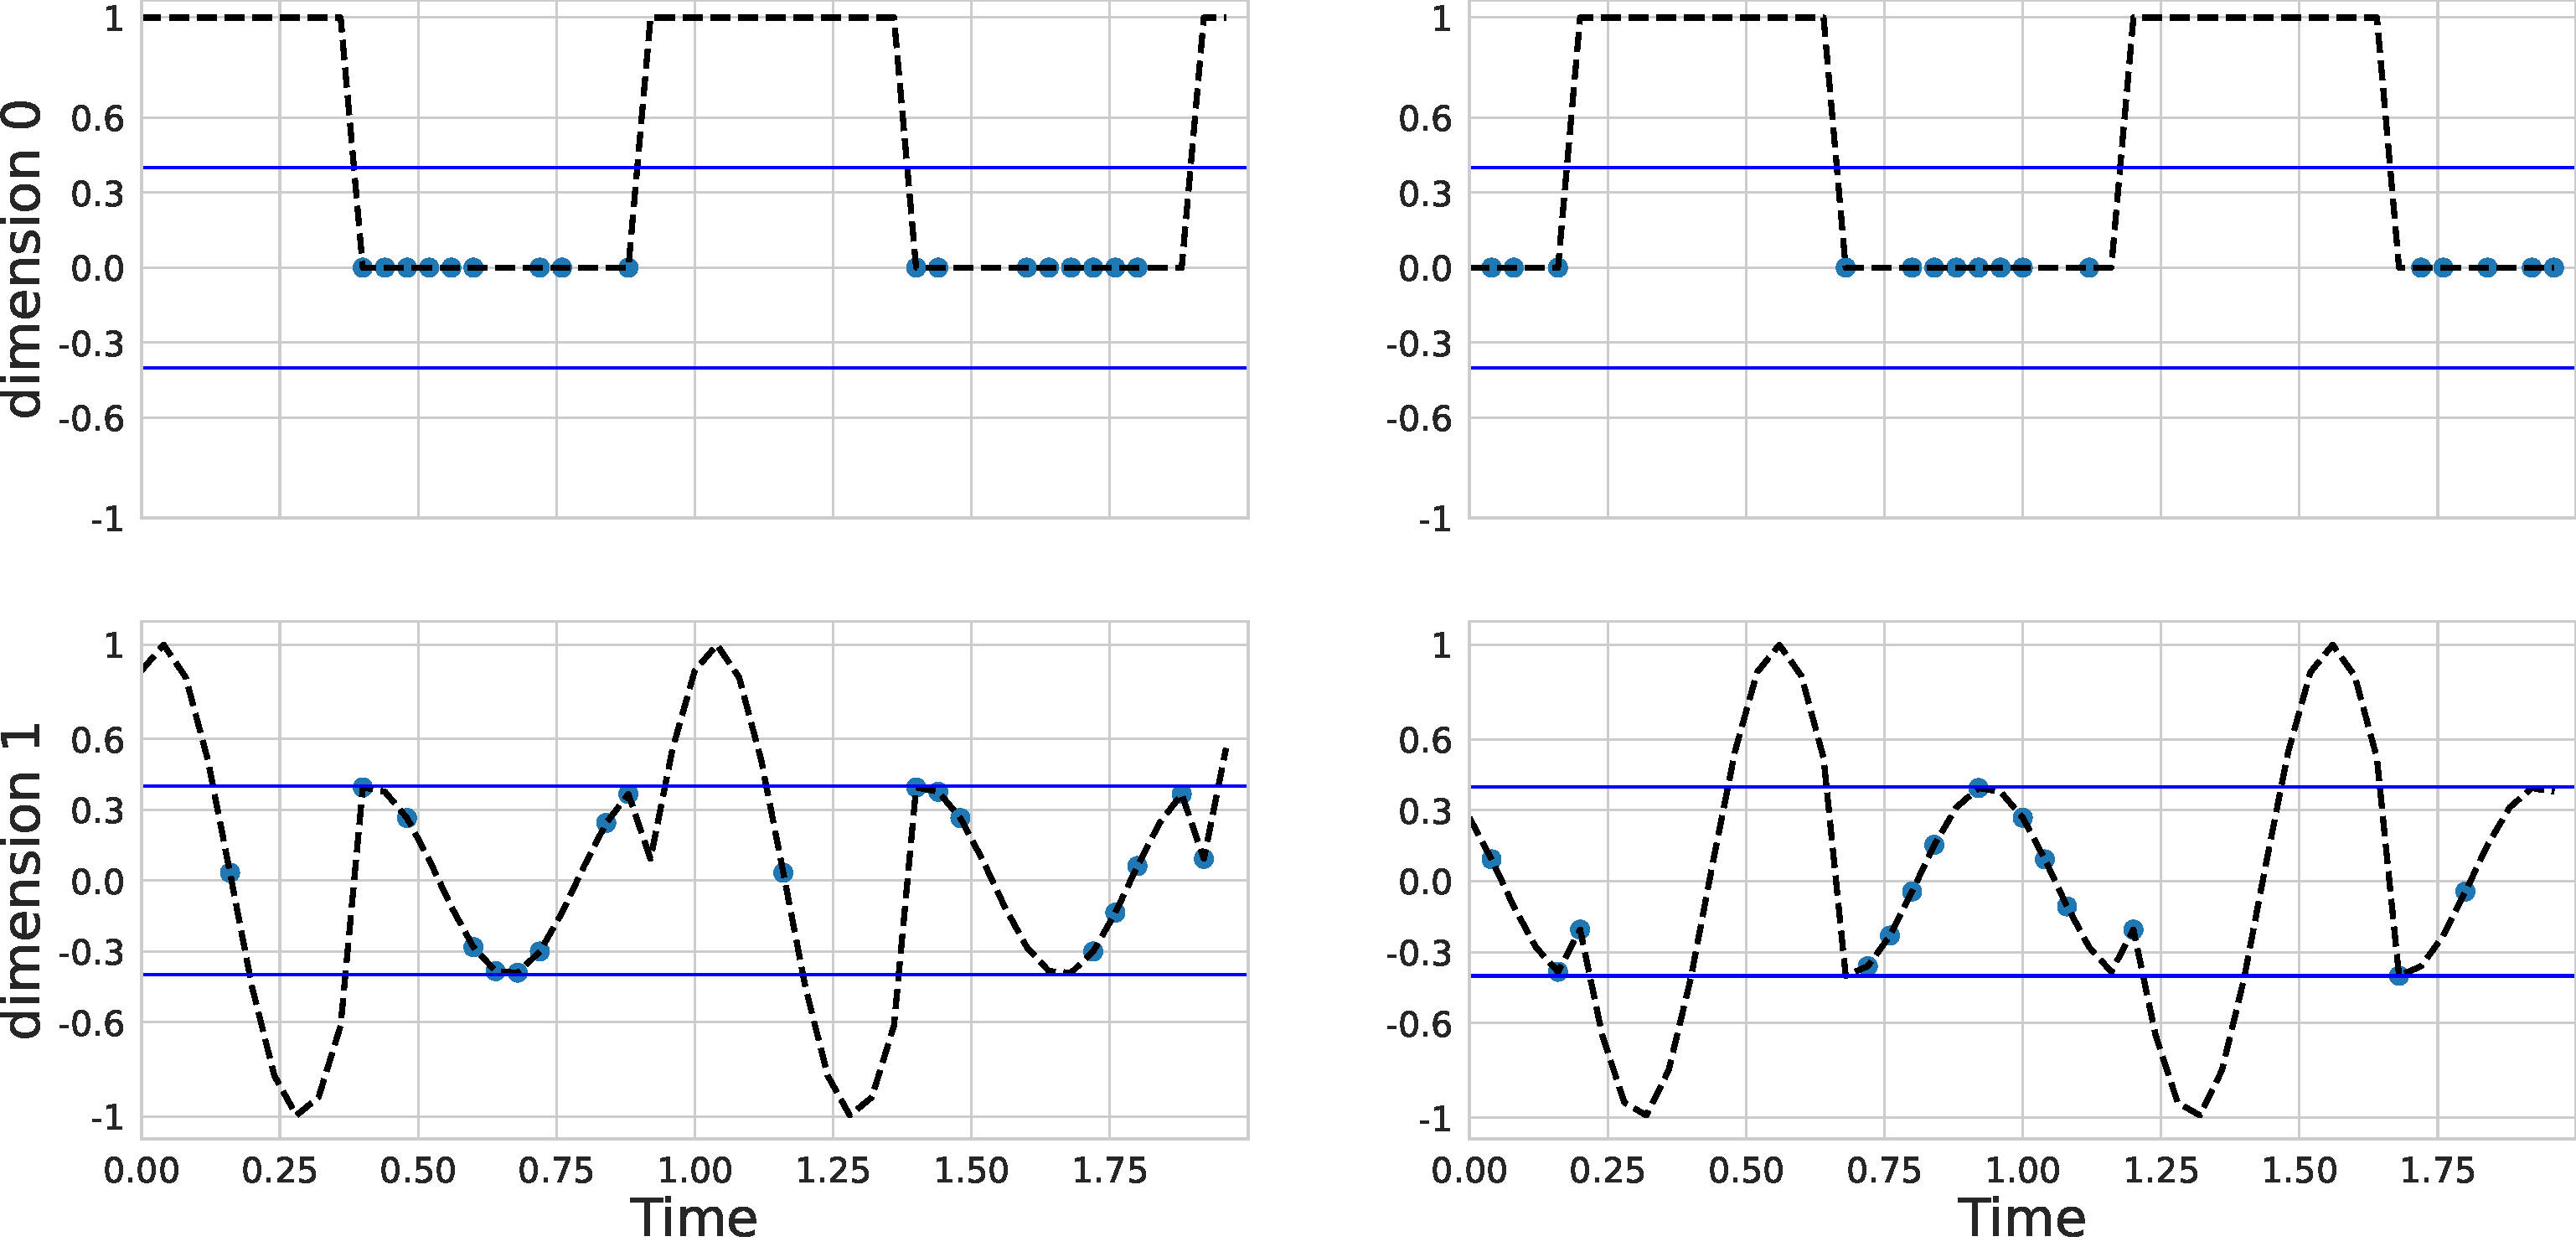
\includegraphics[width=0.9\textwidth]{content/chapters/irregular_time_series_data_driven_missingness/figures/toy_data.pdf}
    \caption[Examples of generated sequences for the synthetic task]{Two examples of generated sequences for the synthetic task. The dashed black lines represent the true data-generating process. The circular dots represent the observations at irregular timepoints. To incorporate data-dependent missingness, the probability of observing a value within the solid blue lines is 0.6; outside the lines is $p_{\text{S}}=0.0006$.}
    \label{fig:toy_example_sequences}
\end{figure}